\documentclass{article}%
\usepackage[T2A,T1]{fontenc}%
\usepackage[utf8]{inputenc}%
\usepackage{geometry}%
\geometry{tmargin=20mm,bmargin=20mm,lmargin=20mm,rmargin=20mm}%
\usepackage{newtxtext, newtxmath}%
\usepackage{substitutefont}%
\usepackage{lastpage}%
\usepackage{gensymb}%
\usepackage{ragged2e}%
\usepackage{graphicx}%
\usepackage{amsmath}%
\usepackage{subcaption}%
\usepackage{fancyhdr}%
%
\linespread{1.5}%
\usepackage{newunicodechar}%
\fancypagestyle{header}{%
\renewcommand{\headrulewidth}{0.5pt}%
\renewcommand{\footrulewidth}{1.0pt}%
\fancyhead{%
}%
\fancyfoot{%
}%
\fancyhead[C]{%
TECHNICAL SCOPE OF WORK%
}%
\fancyfoot[L]{%
H{-}MAC539{-}RFT{-}OE{-}0331{-}001{-}SHT{-}001%
}%
\fancyfoot[R]{%
Page \thepage\ of \pageref{LastPage}%
}%
}%
%
\begin{document}%
\pagestyle{empty}%
\normalsize%
\pagestyle{header}%
\begin{center}%
\section*{}%
\label{sec:}%
\begin{minipage}{\textwidth}%
\centering%
\begin{Large}%
\textbf{MAC MINING AND PARTNERS}%
\end{Large}%
\vspace*{20pt}%
\linebreak%
\begin{large}%
\textbf{RIVER WATER ABSTRACTION}%
\end{large}%
\vspace*{20pt}%
\linebreak%
\begin{large}%
\textbf{H{-}MAC539}%
\end{large}%
\vspace*{20pt}%
\linebreak%
\begin{large}%
\textbf{H{-}MAC539{-}RFT{-}OE{-}0331{-}001{-}SHT{-}001}%
\end{large}%
\vspace*{80pt}%
\end{minipage}

%
\end{center}%
\begin{center}%
\begin{minipage}{\textwidth}%
\flushleft%
\begin{tabular}{|l |l |}%
\hline%
\textbf{Engineer:}&Gerald Holt (Pr.Eng)\\%
\cline{1%
-%
2}%
\textbf{Registration:}&20020259\\%
\cline{1%
-%
2}%
\textbf{Email:}&gerald@holtconsulting.co.za\\%
\cline{1%
-%
2}%
\textbf{Phone:}&+27{-}791{-}2549\\%
\cline{1%
-%
2}%
\textbf{Adress:}&Unit G, Mini Park\\%
\cline{1%
-%
2}%
\textbf{}&16 Gerhardus Street, Strijdom Park\\%
\cline{1%
-%
2}%
\textbf{}&Randburg, South Africa\\%
\cline{1%
-%
2}%
\textbf{Website:}&www.holtconsulting.co.za\\%
\cline{1%
-%
2}%
\end{tabular}%
\vspace*{150pt}%
\centering%
\end{minipage}%
\end{center}%


\begin{figure}[h!]%

\includegraphics[width=240px]{C:/_EEMS/apps/accounts/logos/HCE.jpg}%
\centering%
\end{figure}

%
\newpage%
\begin{center}%
\section*{REVISION HISTORY}%
\label{sec:REVISIONHISTORY}%

%
\begin{minipage}{\textwidth}%
\centering%
\begin{tabular}{|c |c |c |c |c |c |}%
\hline%
\textbf{REV}&\textbf{DESCRIPTION}&\textbf{DATE}&\textbf{ISSUED BY}&\textbf{REVIEWED BY}&\textbf{APPROVED}\\%
\hline%
\end{tabular}%
\end{minipage}%
\end{center}%
\newpage%
\section{CUSTOMER DETAILS}%
\label{sec:CUSTOMERDETAILS}%
\begin{flushleft}%
\begin{minipage}{\textwidth}%
\centering%
\begin{tabular}{|l |l |}%
\hline%
\textbf{Customer:}&Cardinal Namdini Mining Ltd\\%
\cline{1%
-%
2}%
\textbf{Customer Name:}&Bright Dzah\\%
\cline{1%
-%
2}%
\textbf{Customer Email:}&bright.dzah@cardinalresources.com.au\\%
\cline{1%
-%
2}%
\end{tabular}%
\end{minipage}%
\end{flushleft}

%
\newpage%
\section{PROJECT DATA}%
\label{sec:PROJECTDATA}%
\subsection{Applicable Codes}%
\label{subsec:ApplicableCodes}%
\begin{flushleft}%
SANS 10208: Design of structure for the mining industry Part 3: Conveyances%
\linebreak%
SANS 10160: Buidling Loading Code%
\linebreak%
SANS 10162: Steel Design Code%
\linebreak%
SANS 10100{-}1: The Structural use of concrete Part 1 – Design%
\linebreak%
SANS 10100{-}2: The Structural use of concrete Part 2 – Materials and Execution of Work%
\linebreak%
SANS 10144: Detailing of steel reinforcement for concrete%
\linebreak%
SANS 10161: The design of foundations for buildings%
\linebreak%
SANS 110: Sealing components for the building industry, two components, polysulphide base%
\linebreak%
SANS 10164: The structural use of masonry Part 1%
\linebreak%
BS 2853: The design and testing of steel overhead one way beams%
\linebreak%
AWS D1.1: Structural Welding Code {-} Steel%
\linebreak%
SANS 10120{-}3: Corrosion protection systems for steelwork%
\linebreak%
EN 10025: Hot rolled products of structural steel%
\linebreak%
SANS 986: Pre{-}cast reinforced concrete culverts%
\linebreak%
SANS 1077: Sealing compound for the building and construction industry, two components, polyurethane base%
\linebreak%
BS 3148: Test for water for making concrete%
\linebreak%
BS 5075{-}1: Concrete admixtures%
\linebreak%
BS 5075{-}2: Specification for accelerating admixtures, retarding admixtures and water reducing admixtures%
\linebreak%
BS 5075{-}3: Specification for air{-}entraining admixtures%
\linebreak%
BS 5075{-}4: Specification for superplasticizing admixtures%
\linebreak%
BS 5838: Specification for dry packed cementitious mixes%
\linebreak%
BS 5838{-}1: Prepacked concrete mixes%
\linebreak%
BS 5838{-}2: Prepacked mortar mixes%
\linebreak%
\end{flushleft}

%
\subsection{Site Conditions}%
\label{subsec:SiteConditions}%
\begin{flushleft}%
\begin{minipage}{\textwidth}%
\flushleft%
\begin{tabular}{|l |l |c|}%
\hline%
\textbf{Country}&Ghana&\\%
\hline%
\textbf{Region}&Talensi District (Upper East Region of Ghana)&\\%
\hline%
\textbf{Closest Regional Centre}&Bolgatanga&\\%
\hline%
\textbf{Distance to Regional Centre}&50&$km$\\%
\hline%
\textbf{Main Route to Regional Centre}&Talensi Trunk Road off the Tamale{-}Bolgatango Highway&\\%
\hline%
\textbf{Elevation Above Sea Level}&190&$m AMSL$\\%
\hline%
\textbf{Coordinates}&10.63 ° N (Latitude)&\\%
\hline%
\textbf{}&0.66 ° W (Longitude)&\\%
\hline%
\textbf{Area Climate}&Cool, Dry and Dusty&\\%
\hline%
\textbf{Maximum Temperature}&39.3&$°C$\\%
\hline%
\textbf{Average Temperatren}&28.9&$°C$\\%
\hline%
\textbf{Minimum Temperature}&19.3&$°C$\\%
\hline%
\textbf{Maximum Humidity}&68.8&$\%$\\%
\hline%
\textbf{Average Humidity}&46.5&$\%$\\%
\hline%
\textbf{Minimum Humidity}&40.3&$\%$\\%
\hline%
\textbf{Maximum Annual Rainfall}&1464&$mm/a$\\%
\hline%
\textbf{Average Annual Rainfall}&1022&$mm/a$\\%
\hline%
\textbf{Minimum Annual Rainfall}&May to October&\\%
\hline%
\textbf{Maximum Rainfall in 24 hours}&160&$mm$\\%
\hline%
\end{tabular}%
\end{minipage}%
\end{flushleft}

%
\newpage%
\subsection{Sketches and Drawings}%
\label{subsec:SketchesandDrawings}%
\subsubsection{Basic Flow Diagram}%
\label{ssubsec:BasicFlowDiagram}%


\begin{figure}[h!]%
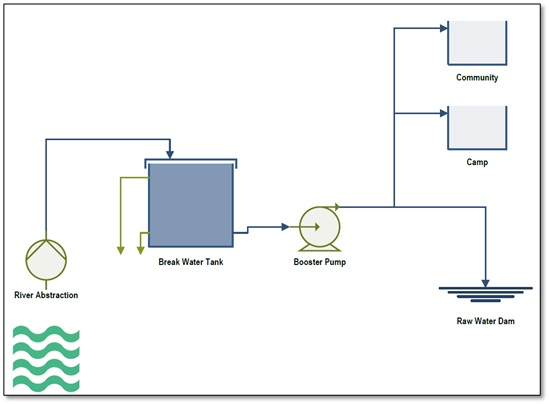
\includegraphics[width=450px]{C:/_EEMS/apps/documents/tenderSOW/images/BasicFlowChart.jpg}%
\centering%
\caption{Basic Flow Diagram}%
\centering%
\end{figure}

%
\subsubsection{General Layout}%
\label{ssubsec:GeneralLayout}%


\begin{figure}[h!]%
\begin{subfigure}[b]{0.45\linewidth}%
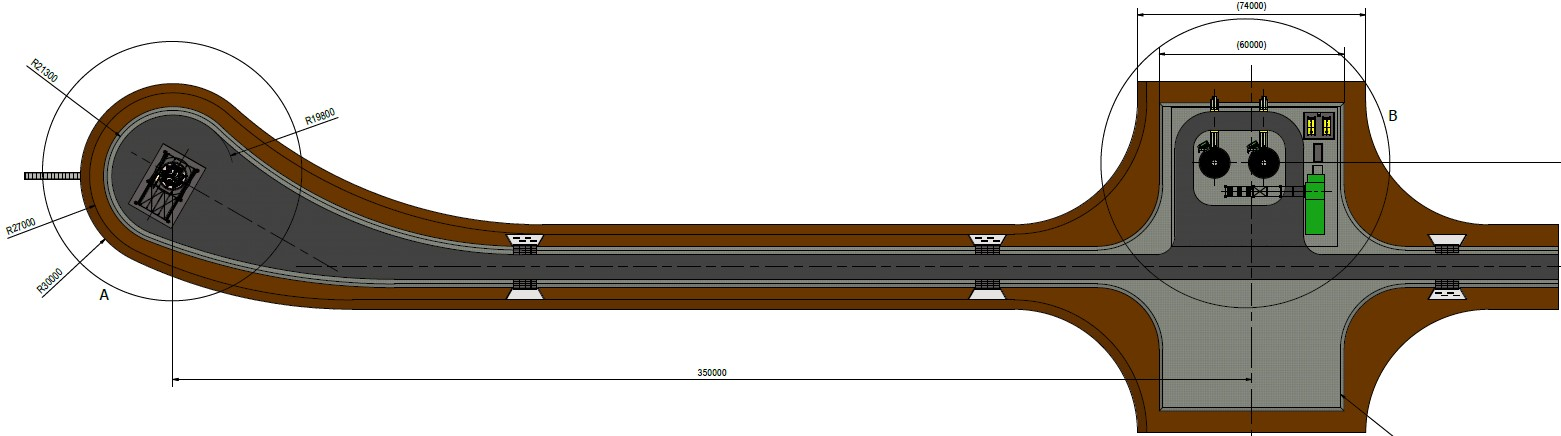
\includegraphics[width=500px]{C:/_EEMS/apps/documents/tenderSOW/images/OverallLayout.jpg}%
\centering%
\caption{Overall River Abstraction Layout}%
\end{subfigure}%
\end{figure}

%
\newpage

%
\subsubsection{River Abstraction Detail}%
\label{ssubsec:RiverAbstractionDetail}%


\begin{figure}[h!]%
\begin{subfigure}[b]{0.45\linewidth}%
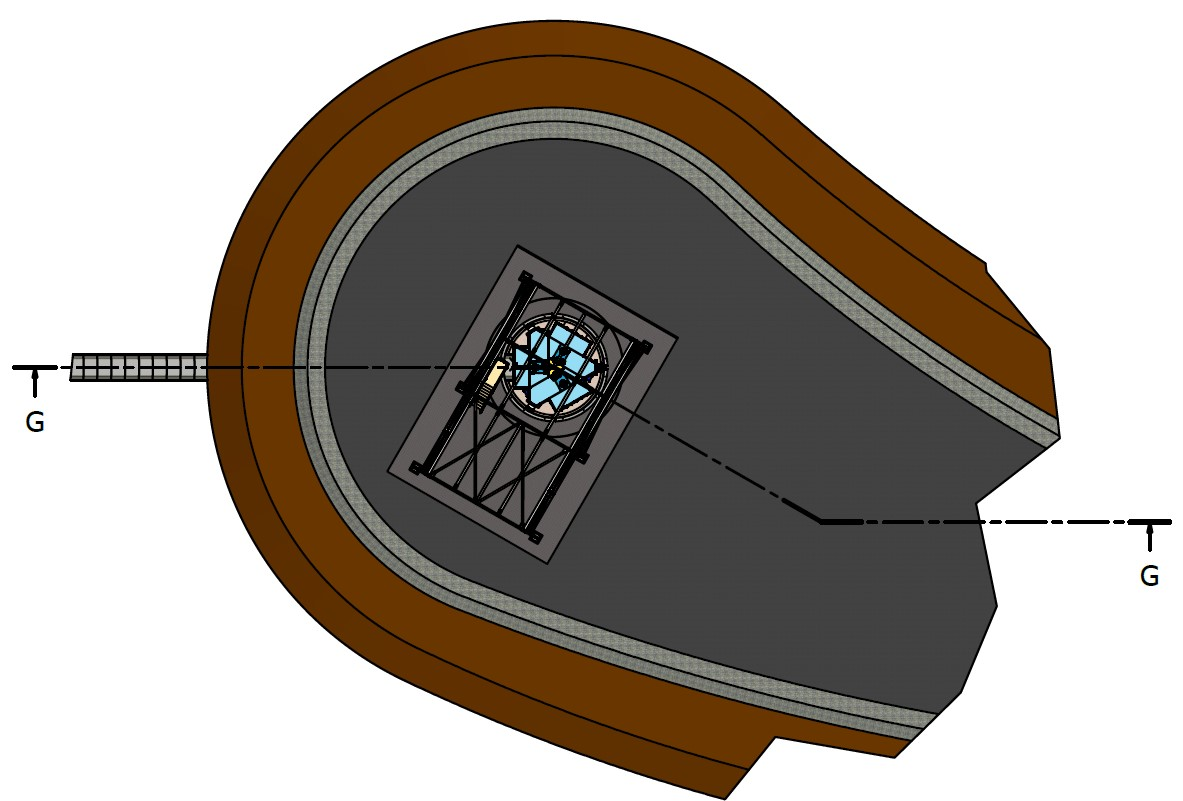
\includegraphics[width=500px]{C:/_EEMS/apps/documents/tenderSOW/images/RiverAbstract1.jpg}%
\centering%
\caption{River Abstraction Detail 1}%
\end{subfigure}%
\end{figure}

%


\begin{figure}[h!]%
\begin{subfigure}[b]{0.45\linewidth}%
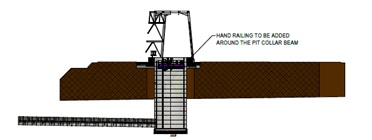
\includegraphics[width=500px]{C:/_EEMS/apps/documents/tenderSOW/images/RiverAbstract2.jpg}%
\centering%
\caption{River Abstraction Detail 2}%
\end{subfigure}%
\end{figure}

%


\begin{figure}[h!]%
\begin{subfigure}[b]{0.45\linewidth}%
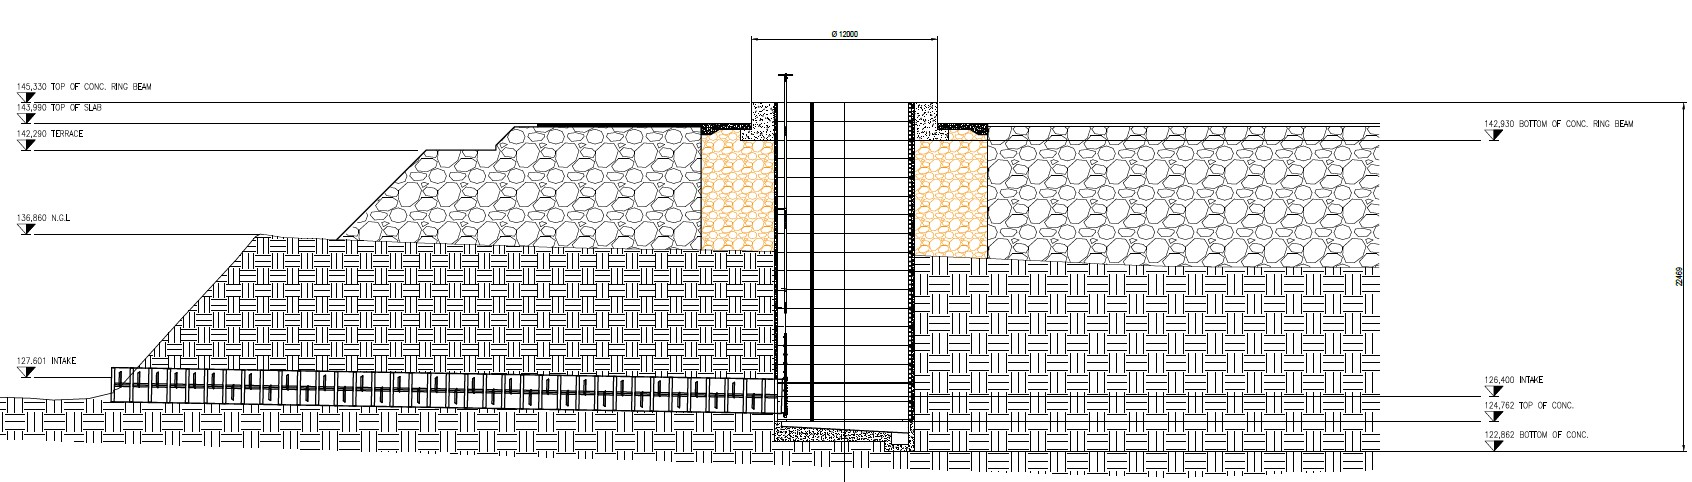
\includegraphics[width=560px]{C:/_EEMS/apps/documents/tenderSOW/images/RiverAbstract3.jpg}%
\centering%
\caption{River Abstraction Detail 3}%
\end{subfigure}%
\end{figure}

%


\begin{figure}[h!]%
\begin{subfigure}[b]{0.45\linewidth}%
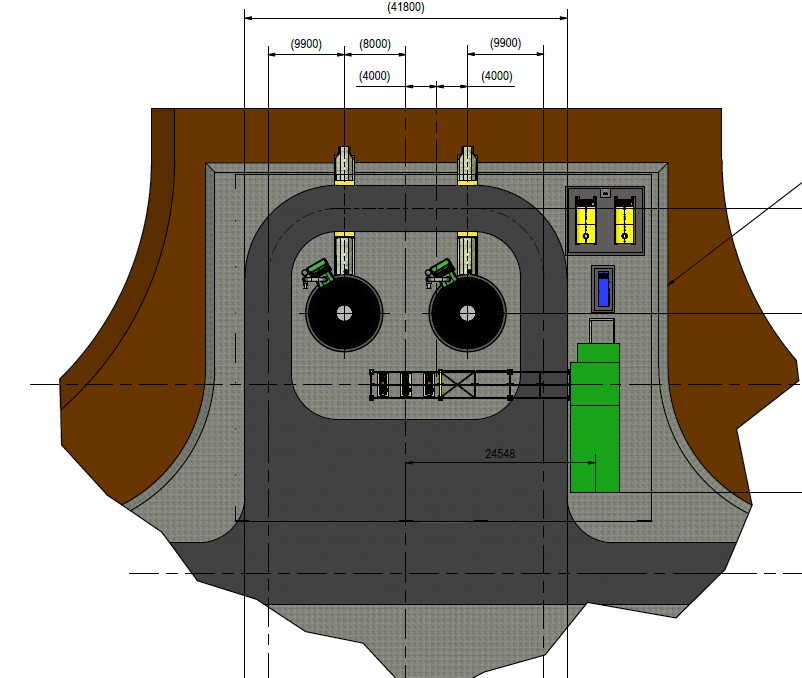
\includegraphics[width=500px]{C:/_EEMS/apps/documents/tenderSOW/images/Booster.jpg}%
\centering%
\caption{Booster Station}%
\end{subfigure}%
\end{figure}

%
\newpage%
\section{PROJECT INFORMATION}%
\label{sec:PROJECTINFORMATION}%
\subsection{Introduction}%
\label{subsec:Introduction}%
Namdini is approximately 50 km southeast of the regional town of Bolgatanga in Northern Ghana and around 60 km south of the Burkina Faso border (Figure 19). Namdini lies within the Nangodi Greenstone Belt, one of a series of southwest–northeast trending granite-greenstone belts which host significant gold mineralization in Ghana and Burkina Faso.
The Talensi district which was part of the Talensi-Nabdam district became a separate district in 2012, through Legislative Instrument LI 2110, with Tongo as the capital. The district, which is one of the thirteen Municipalities and Districts in the Upper East Region, is bordered to the north by the Bolgatanga Municipality, to the south by West and East Mamprusi Districts (both in the Northern Region), to the west by Kassena-Nankana District, and to the east by the Bawku West and Nabdam Districts. The district lies between latitude 10° 15' and 10° 60' North of the equator and longitude 0° 31' and 1° 05' West of the Greenwich Meridian and covers a land area of 838.4 km2 with a total population of 81,194, which constitutes 7.8% of the regional population. It is made up of 96 towns and villages with a settlement pattern which is predominantly rural.
The topographic relief within the project area is generally flat with gently undulating terrain, rising to the south where the area is overlain by sediments. Elevation varies from 175 to 250 meters above mean sea level (“AMSL”) with average elevation at approximately 190 m. Physiography is primarily savannah grassland characterized by short, scattered drought-resistant trees, scrub, and grass that is seasonally burned by bushfires or scorched by the sun during the long dry season.%
\newline%
%
\newline%
%
As part of the water requirements for the process plant, river water abstraction is one of the methods that will be used to supply water to the plant as well as for the camp and accommodation area. The point of abstraction has been identified which is 10,910 meters from the plant. 
Water will be abstracted by means of vertical spindle pumps, which will discharge into breakwater tanks of the booster station, 350 meters from the river in a northern direction. The booster station will accommodate the diesel generator, MCC, diesel storage, and the booster pumps which will transfer the water to the raw water storage. 
Except for areas above ground and the abstraction point, all the piping will be HDPE piping buried next to the main road to the process plant.  Piping passing underneath the main road will also be constructed from steel. The line will be equipped with valve boxes and vacuum breakers as well as the necessary scour points. Also, along the line, a T-off will be installed for the supply line to the camp.

%
\subsection{River Abstraction}%
\label{subsec:RiverAbstraction}%
The point of abstraction is provided by the client. The coordinates of the abstraction point are X=748698.3955, Y=1178401.56, Z= 144.569 (cartesian system). This position was selected as it is the highest point along the river. This is important to accommodate the river level fluctuations and to ensure that the abstraction system is able to perform under these different conditions.%
\newline%
%
\newline%
%
 The following are the attributes of the river abstraction configuration:%
\begin{itemize}%
\item%
The catchpit centre is 45 meters from the riverbank. This distance has been increased from 20 meters to 45 meters to allow space for the causeway, access turning radius and soil stability.%
\item%
The level of the slab around the catch pit is at 143,990 mASL. The top of the catch pit ring beam is 145,330 mASL.%
\item%
Once the abstraction pump chamber earth, civil, and mechanical works are completed, the embankment left in situ to river to be removed during low level conditions of river. The section of soil embankment to be removed after construction of pump chamber must be stabilized by gabions.%
\item%
The centre of the inlet of the water intake pipe is at level 127,600 mASL. Note that the intake slope has been changed to the opposite of that of the original conceptual design. The intake water pipe slopes at 1° downward to the bottom of the catch pit bottom. The centre of the pipe enters the pit at level 126,400 mASL.%
\item%
As the area between transfer pump station and river embankment will flood due to its low elevation, a causeway (complete with culverts to allow water flow) has been incorporated for access to abstraction pumps.%
\item%
The power supply to abstraction pumps to run on the causeway.%
\ldots%
\end{itemize}

%
\subsection{Booster Station}%
\label{subsec:BoosterStation}%
The point of abstraction is provided by the client. The coordinates of the abstraction point are X=748698.3955, Y=1178401.56, Z= 144.569 (cartesian system).%
\newline%
%
\newline%
%
The following are the attributes of the booster station configuration:%
\begin{itemize}%
\item%
The station consists of two areas. On the western side of the causeway is the booster station and on the earstern side the contractor's laydown area.%
\item%
The booster pump station will house the buffer tanks, booster pumps and substation.%
\item%
The area will also be equipped with a building consisting of a security office, control room, store room, workshop and the substation%
\ldots%
\end{itemize}

%
\newpage

%
\end{document}